\documentclass[12pt]{article}
\usepackage[utf8]{inputenc}
\usepackage[a4paper, margin=1in]{geometry}
\usepackage{titlesec}
%\usepackage[style=ieee, backend=biber]{biblatex}
\usepackage{graphicx}
\usepackage{amsmath}
\usepackage{amssymb}
\usepackage{amstext}
\usepackage{enumitem}
\usepackage{siunitx}
\usepackage{array}
\usepackage{xcolor}
\usepackage{multirow}
\usepackage{hyperref}
\usepackage{tabularx}
\usepackage{booktabs}
\usepackage{soul}
\usepackage{fancyhdr}
\usepackage{wrapfig}
\usepackage{setspace}
\usepackage{multicol}
\setlength{\columnsep}{.7cm}

\hypersetup{
    colorlinks=true,
    linkcolor=blue,
    filecolor=magenta,
    urlcolor=blue,
    pdftitle={aes670hw2},
    pdfpagemode=FullScreen,
    }
\urlstyle{same}

\newcolumntype{L}{>{$}l<{$}}  % Math mode table
\newcolumntype{R}{>{$}r<{$}}  % Math mode table
\newcolumntype{C}{>{$}c<{$}}  % Math mode table

\pagestyle{fancy}

\renewcommand{\sectionmark}[1]{%
\markboth{\thesection\quad #1}{}}
\fancyhead{}
\fancyhead[L]{\leftmark}
\fancyfoot{}
\fancyfoot[C]{\thepage}

\bibliographystyle{ieeetr}

\definecolor{Light}{gray}{.9}
\sethlcolor{Light}

\newcommand{\hltexttt}[1]{\texttt{\hl{#1}}}

\newcommand*{\problem}[2]{
    \begin{table}[ht]
    \centering
        \begin{tabular}{ | p{.1\linewidth} p{.9\linewidth} | }
            \hline
            \vspace{.3em}\textbf{\large#1:} & \vspace{.3em}\footnotesize{#2}\hspace{.2em}\vspace{.5em} \\ \hline
        \end{tabular}
    \end{table}
}

\newcommand\T{\rule{0pt}{2.6ex}}       % Top strut
\newcommand\B{\rule[-1.2ex]{0pt}{0pt}} % Bottom strut

\titleformat{\section}
  {\normalfont\fontsize{12}{13}\bfseries}{\thesection}{1em}{}

\titleformat{\subsection}
  {\normalfont\fontsize{12}{15}\bfseries}{\thesubsection}{1em}{}

\begin{document}

%\maketitle

{\large\begin{center}\textbf{Deep Learning Methods for Estimating 1km Broad-band TOA Flux with CERES and MODIS Imagery}\end{center}}

{\begin{center}\textbf{Mitchell Dodson}\end{center}}

    \vspace{-1em}
\section{Introduction}
\vspace{-1em}

Satellite observation of broad-band outgoing longwave and shortwave radiance is an indespensible resource for understanding Earth's energy budget thanks to the unparalleled spatial coverage of in-orbit radiometers, and their ability to directly measure the directional solar reflectance and thermal emissions from an entire atmospheric path. These properties make them a vital basis for evaluating atmospheric and land surface reanalysis datasets like ERA5 \cite{loeb_evaluating_2022}, reducing error in surface-based bulk flux approximations \cite{yu_global_2019}, investigating the extent and theoretical fidelity of climate feedbacks like clouds and aerosols \cite{ramanathan_cloud-radiative_1989}\cite{zhang_longwave_2003}, and characterizing the radiative effects of large-scale phenomena like the El Ni\~no Southern Oscillation processes and poleward atmospheric energy transport \cite{loeb_observing_2014}\cite{mayer_poleward_2012}.

Nonetheless, satellite-based instruments measuring wide-band radiance generally have coarse spatial resolution on the order of tens of kilometers in order to maintain sufficient precision over the full range of their spectral response. This is in spite of the fact that many features that have a considerable impact on Earth's energy budget like clouds, urban development, and variations in vegetation type and coverage have characteristic scales which are often much smaller. Modern satellite projects like the NASA Earth Observation System (EOS), Suomi NPP, and JPSS which support wide-band instruments also typically provide data in narrow visible and infrared bands at a much finer resolution. While previous studies have used statistical regression techniques to merge multi-instrument observations of a scene into data products estimating TOA flux at finer resolutions \cite{wang_estimating_2016}\cite{loeb_fusion_2006}, there is general a lack of investigation of deep learning methods that may be suited to the task (with one exception, addressed later \cite{li_evaluation_2022}). As such, in this document I make the argument that unsupervised methods for machine learning are appropriate for extracting spatial and spectral characteristics of imager observations that are relevant for estimating TOA flux, and propose a novel approach for training several deep learning models with the end-goal of developing a 1km TOA shortwave and longwave flux product based on MODIS data.

\vspace{-1em}
\section{Satellites and Earth's Radiation Budget}
\vspace{-1em}

The value of satellite observations of outgoing radiation was recognized early in the devopment of space technology, with the first estimates of global shortwave and longwave fluxes being derived from the TIROS and ESSA III platforms in the late 1960s \cite{house_radiation_1965}\cite{vonder_haar_satellite_1969}. These efforts were formalized with the launch of broad-band Earth's Radiation Budget (ERB) instruments alongside Advanced Very High Resolution Radiospectrometer (AVHRR) imagers aboard a constellation of polar-orbiting satellites including Nimbus 7, NOAA-9, and NOAA-10 \cite{barkstrom_earth_1984}. The ERB instruments offered a high signal-to-noise ratio across a wide spectrum in the shortwave ($.2-5\,\si{\mu m}$) and longwave ($5-50\,\si{\mu m}$) regions, and the AVHRR instruments provided 4-6 bands with spatial resolution at $4\,\si{km}$, or $1\,\si{km}$ on a limited domain \cite{shenk_noaa-10_nodate}.

\begin{figure}[h!]
    \centering

    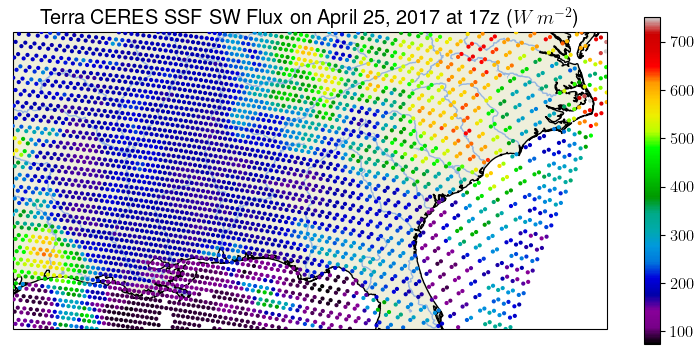
\includegraphics[width=.33\linewidth]{figs/swflux.png}
    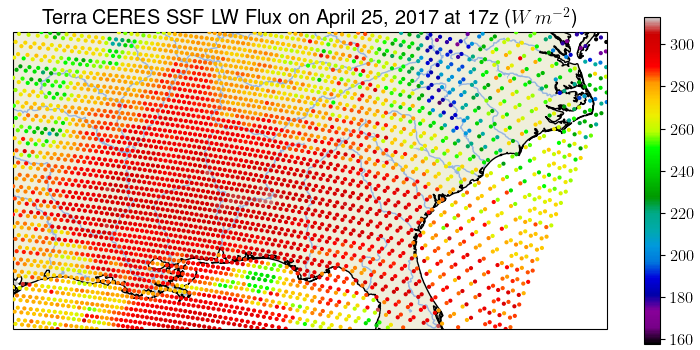
\includegraphics[width=.33\linewidth]{figs/lwflux.png}
    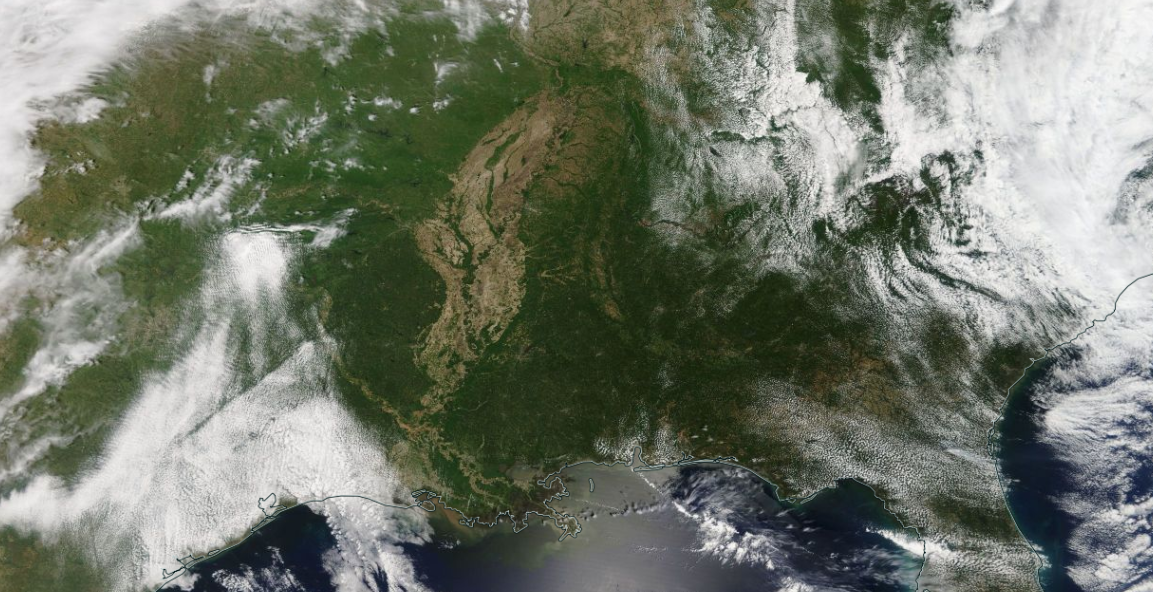
\includegraphics[width=.32\linewidth]{figs/modis.png}

    \caption{Comparison between shortwave and longwave flux from CERES Single Scan Footprint (left and middle), and cotemporal MODIS truecolor imagery (right) over the field of regard for this project. The bulk influence of clouds and land-surface features is apparent in the CERES footprint data, for example the increase in outgoing shortwave and depression in outgoing longwave radiation associated with the cloud deck over Virginia, however kilometer-scale features like the cumulus clouds over Florida are only distinguishable in the MODIS imagery.}
    \label{cover}
\end{figure}

Following the success of the ERB experiment, the Clouds and Earth's Radiant Energy System (CERES) instrument aboard the Terra and Aqua satellites has provided a near-continuous data record of top-of-atmosphere (TOA) broad-band fluxes for over two decades. CERES has three channels in the shortwave ($.3-5.0\,\si{\mu m}$) window ($8.0-12.0\,\si{\mu m}$) and total-spectrum ($.3-200\,\si{\mu m}$) ranges, which allow for measurement of solar reflectance and terrestrial emission with and an overall precision up to three times that of the ERB instruments within an elliptical receptive area (footprint) varying between about $20\,\si{km^2}$ and $40\,\si{km^2}$ depending on the panoramic distortion at the viewing angle \cite{wielicki_clouds_1996}. The Terra and Aqua satellites also include Moderate Resolution Imaging Spectroradiometer (MODIS) instruments that contribute 36 narrow spectral bands distributed throughout the $0.41-14.1\,\si{\mu m}$ range with nadir resolutions of $1\,\si{km^2}$ or finer.

The juxtaposition of imager data having fine spatial/spectral resolution with radiometers providing broad-spectrum shortwave/longwave radiance proved a critical innovation that facilitated the development of Angular Dependence Models (ADMs), which considerably improve the reliability of full-sky TOA flux estimates. In particular, ADMs are lookup tables that use averages derived from large ensembles imager data to characterize the distribution of radiance reflected and emitted by a certain surface type given a specific sun/pixel/satellite geometry \cite{suttles_angular_1988}\cite{loeb_angular_2005}. This is necessary for an accurate understanding of the overall energy budget because many surfaces are strongly anisotropic, so the assumption that the radiance observed for a feature is linearly proportional to the total hemispherical exitance doesn't often hold.

In practice, the surface type of an imager pixel is discretely determined by comparing its spectral properties in multiple bands to clusters of similar pixels, then the table associated with the selected surface type is inverted using the scene's angular geometry to select an anisotropic factor. This coefficient is finally used to scale the radiance to an estimate of the radiant flux integrated over all viewing angles, which is the quantity most directly related to Earth's energy budget. Since the imager pixels used to determine incident surface types have a much finer spatial resolution than the broadband footprints from which flux measurements are derived, the footprints often contain a mixture of multiple surface types. Therefore, the anisotropic factors used to determine flux values associated with a broadband observation are generally calculated as an average of the imager properties, which is spatially weighted by the Point Spread Function (PSF) of imager pixels in the receptive area with respect the footprint's centroid.

\vspace{-1em}
\section{Regression Strategies in Machine Learning}
\vspace{-1em}

Machine learning describes a broad category of powerful constructs for iteratively developing a representation of the intrinsic properties and relationships between complex datasets. At a fundamental level, most machine learning algorithms function by accepting an arbitrary-dimensional numerical vector as an input, then composing a series of learned affine matrix transformations (hidden layers), each followed by element-wise operations that are differentiable but nonlinear (activation functions). Ultimately, the model produces an arbitrary-dimensional vector as an output. During the training process, a large volume of input samples are individually transformed by the model's hidden layers until the vector of output values (prediction) is arrived at. The prediction is subsequently compared to the ideal output corresponding to the input sample by a loss function which characterizes the skill of the model for evaluating that sample.

Since the affine transformation and element-wise activation function are necessarily differentiable at each layer of the model, the chain rule can be used to determine the output vector's gradient of sensitivity with respect to each element of the affine transformation matrix at every layer starting with the closest one to the output. Provided this distribution of sensitivity values throughout the model, an optimization algorithm is used to systematically adjust the matrix element values -- which constitute the learned weights and biases of the model -- such that the total error over collections of input samples is progressively reduced \cite{russell_artificial_2010}\cite{srivastava_highway_2015}. When multiple hidden layers are used, the model gains the capacity to learn increasingly sophisticated and nonlinear abstractions, which is a now-ubiquitous approach known as deep learning \cite{lecun_deep_2015}.

In contemporary times, much of the progress in data science applications for deep learning models involves developing novel high-level architectures built on top of the same basic principles outlined above. By modulating the depth and breadth of connections between layers and by introducing regular sub-structures, and flow of information and error through the model can be optimized for a particular domain of problems. For example, Convolutional Neural Networks (CNNs) are a category of model architectures that is currently very popular for problems involving data which is gridded on two or more orthogonal axes.

Rather than learning a single large vector of weights which are applied to the entire input sample simultaneously, the CNN strategy entails learning weights that constitute a series of kernel grids that are generally much smaller than the input layer. The kernels are typically learned independently to each other by convolving their weights over the input grid to generate the next layer of activations. This approach is useful because imbues the model with translation-invariance to input data and encodes a default spatial scale over which the kernels are receptive \cite{lecun_gradient-based_1998}.

All of the prior literature I found that applies deep learning techniques to MODIS data with the goal of producing broad-band fluxes utilized architectures derived from CNNs. Li et al. implemented CNN-based Deep Belief Networks and ResNet models with multiple kernel sizes, and used ERA5 reanalysis data as a truth basis. While their models were successful in producing consistent fine-resolution flux estimates based on ERA5 reanalysis data, the outputs are limited to daily estimates of net radiative flux rather than instantaneous observations \cite{li_evaluation_2022}. Zhan et al generated a 21-year dataset of TOA 1km longwave fluxes based on MODIS data with respect to CERES observations that have been resampled onto a regular grid using bilinear interpolation. Their technique employed a gradient-boosted regression network similar to a CNN architecture which showed impressive skill in validation \cite{zhan_generation_2023}. Nonetheless, there are several shortcomings that arise due to the method's reliance on a gridded dataset. First, CNN-like architectures require that the input conforms to a fixed grid shape. This means that the MODIS data used to initialize the model as well as the flux data used as a truth basis need to be re-sampled onto large and regular image grids in order to train and execute the model. This is appropriate for some applications, however it limits the utility of the architecture as an analysis tool for investigating the direct correspondence between MODIS imagery and outgoing flux. Furthermore, the resampling process may contaminate the comparison between CERES fluxes and MODIS pixels since the radiative effects of sub-footprint features such as cloud edges are extrapolated over a wider area than the corresponding MODIS pixels would actually represent.

In addition to the gridded problem domains most commonly accommodated by CNNs, machine learning is also widely adapted to a sequence-to-sequence (seq2seq) problem type, which entails a model architecture that accepts and produces a number of fixed-length vectors. Common applications for seq2seq problems include natural language processing and time series regression, both of which benefit in many cases from the flexibility to accept variable-length inputs, and from the capacity to reference the full context of the input sequence while generating the output. The specific architectures applied to seq2seq problems vary widely, however two rather different strategies of interest for this project which boast both of these abilities are Long Short-Term Memory networks (LSTMs) and Transformer models.

\begin{wrapfigure}{r}{.5\linewidth}
    \begin{center}
        \vspace{-2.5em}
        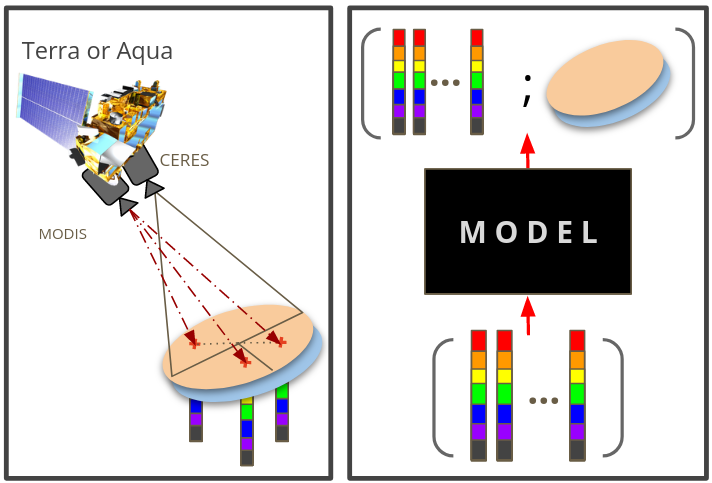
\includegraphics[width=.95\linewidth]{figs/schematic.png}
        \caption{Schematic diagram demonstrating how estimation of outgoing flux from MODIS pixels co-located with CERES data can be posed as a sequence-to-sequence regression problem using an autoencoder-like deep learning model.}
        \vspace{-1.5em}
        \label{schematic}
    \end{center}
\end{wrapfigure}

Since CERES single-scan footprints don't reliably conform to a fixed grid, but have receptive areas that can be directly associated with near-simultaneous MODIS observations, I'm proposing to reformulate the problem as a seq2seq-style regression, with each input and output sequences consisting of a collection of MODIS pixel vectors clustered around a single CERES footprint's centroid. This has several advantages, namely that (1) since neither the CERES flux footprints nor the MODIS pixels have been re-gridded, there is a more direct correspondence between observations by the two instruments, with fewer artifacts from interpolation, (2) relieving the dependence on a fixed grid would make the model more useful as an analysis tool since small subsets of MODIS pixels may be processed independently from an entire granule, and (3) while spatial features on the ~20km native scale of a CERES footprint will be initially learned inputs at the default MODIS resolution, the freedom to train on variable-length inputs lends itself to fine-tuning the model on sparse data, or even different datasets with entirely different resolutions.

LSTMs are a style of Recurrent Neural Network (RNN), which implies that they apply a consistent sub-structure to each element of the input or output sequence using the same learned weights. For each additional element in the sequence, the activation values from the previous element are passed to the recurrent component, allowing for the propagation of a so-called context vector containing information from the previous inputs. Since the same weights are used for each element, it's generally straightforward and efficient to train models to be agnostic to the length of the sequence and to accept skipped data values using basic masking techniques. LSTMs advance this concept by maintaining a context vector that is only operated on indirectly and element-wise by the input sequence via the activations from 3 learned information gates. This improves the stability of the network over long sequences since the persisting information isn't transformed by a matrix operation after every element. \cite{hochreiter_long_1997}\cite{vennerod_long_2021}

Transformers are a more recent approach to seq2seq problems which have achieved impressive new states of the art in many use cases. Unlike RNN-based seq2seq architectures, transformers accept the entire input sequence at once, and apply an innovative technique called multi-headed attention (MHA) in order to make predictions by dynamically focusing on different parts of the input \cite{vaswani_attention_2017}. Although transformers are especially well-known for their aptitude in solving NLP problems, they have been adapted to computer vision tasks with great success and have been shown to be skillful in learning spatial properties of input data \cite{dosovitskiy_image_2021}\cite{he_masked_2021}.

As a final piece of context, all of the above machine learning model varieties can be pre-trained in an unsupervised fashion as autoencoders. An autoencoder is an architecture which initially learns to reduce the input data to a vector representation that is much smaller than its original size, then re-produces the input with the highest possible fidelity. If the model is reliably skillful in generating the original data after having its degrees of freedom substantially reduced, then the intermediate vector, known as the latent space representation, must have properties that correspond to abstract and expressive qualities of the original dataset. \cite{quade_sparse_2018}\cite{kashinath_physics-informed_2021}\cite{gao_bayesian_2022} Once the autoencoder is trained, the portion of the model that decodes the intermediate representation is discarded and replaced by a new and untrained decoder, which subsequently learns to accept the information-rich latent vector from the encoder as an input, and translate it into an output that has properties correlated with the characteristics extracted and generalized from the original data.

\vspace{-1em}
\section{Methodology}
\vspace{-1em}

\begin{wrapfigure}{r}{.6\linewidth}
    \centering
    \begin{tabular}{| c c c |}
        Band & Wavelength ($\mu m$) & Role \\
        \hline
        8 & .41 & Near UV \\
        3 & .46 & Blue \\
        4 & .55 & Green \\
        1 & .64 & Red \\
        2 & .86 & Near-Infrared \\
        18 & .935 & NIR Water Vapor \\
        26 & 1.38 & Cirrus \\
        6 & 1.64 & Cloud Phase \\
        7 & 2.11 & Particle Size \\
        20 & 3.7 & Shortwave IR \\
        27 & 6.5 & Upper Water Vapor\\
        30 & 9.7 & Ozone \\
        31 & 10.9 & Clear IR Window \\
        33 & 13.3 & CO$_2$ \\
    \end{tabular}
    \caption{MODIS bands used as input features for model training.}
\end{wrapfigure}

Throughout this project I aim to develop and compare a series of autoencoder networks based on the LSTM and transformer architectures which will initially learn to reproduce the spatial and spectral features from MODIS pixels embedded in a circular domain surrounding the center of CERES footprints. In each case, this will be accomplished using a progressive masking strategy by which two encoders will be separately trained for each architecture. The first will encourage the training process to learn to make spatial generalizations within the receptive areas by interpolating onto an increasing number of masked sequence elements, and the second will similarly learn to interpolate spectral features within individual samples by randomly masking an increasing number of bands. Once the models prove skillful in re-generating the input sequence, the latent vector outputs will be concatenated, and a new decoder head will be trained to output separate shortwave and longwave flux values corresponding to each pixel, optimizing the similarity between the average of all pixels in the sequence and the flux values from the corresponding CERES footprint. This approach is similar in spirit to several recent papers  which show that employing dual-branch spatial and spectral modules make autoencoder-like architectures more robust for hyperspectral classification and segmentation tasks. \cite{praveen_novel_2019}\cite{praveen_bidirectional_2022}\cite{praveen_dual-branch-attentionnet_2022}


\begin{enumerate}[itemsep=0pt, parsep=0pt, before=\setlength{\baselineskip}{6mm}]
    \item Download MODIS L1b imager data and CERES SSF longwave and shortwave fluxes for 2015, 2017, 2019, and 2021 within a region covering the South East US.
    \item For each of N CERES footprints in a satellite overpass (swath), collect the nearest K MODIS imager pixels. Encode their position as the great circle distance and azimuth to the CERES centroid.
    \item Store each swath as a (N,1,C) array of C CERES features, and a (N,K,M) array of M MODIS features, each along with a list of strings labeling each feature axis.
    \item Quality-check the data by making sure there are no NaN values or data outside of the acceptable range. Remove any swaths that have no valid data from the dataset.
    \item Gauss-normalize all in-range data and collect it into memory-mapped arrays for training and validation data.
    \item Train an LSTM based autoencoder model to reproduce a sequence of up to K of the nearest imager pixels, optimizing for spatial interpolation by sparsely masking sequence elements.
    \item Train an LSTM based autoencoder model optimizing for spectral interpolation by masking feature elements.
    \item Develop a decoder head that converts the combined latent-space output of both above models into an estimate of the longwave and shortwave flux contribution of each MODIS pixel, using a custom loss function that compares the spatial average of pixel values to the bulk CERES footprint values for flux.
    \item Repeat steps 6-8 using the same dataset and training strategy, except using a transformer architecture.
\end{enumerate}


\newpage

\bibliography{main}

\end{document}

\begin{table}[h!]
    \centering
    \begin{tabular}{ m{.15\linewidth} | m{.15\linewidth} | m{0.6\linewidth}}
        \textbf{Parameter} & \textbf{Value} & \textbf{Justification} \\
        \hline
        & & \\
    \end{tabular}
    \caption{}
    \label{}
\end{table}

\begin{table}[h!]\label{}
    \centering
    \begin{tabular}{ c c | c c c c c}
        & & & & & & \\
        \hline
        \multirow{4}*{} &
        & & & & & \T\\
        & & & & & \B\\
        \hline
        \multirow{2}*{Valid} &
        Meta & .2779 & .246 & .3684 & .4755 & .3923 \T\\
        &Grid & .2791 & .2495 & 2.270 & 2.378 & 2.292 \B\\
    \end{tabular}
    \caption{Comparison between my retrieval results and AOD values reported in the DESIS metadata, as well as the pixels in the AOD tiff grid corresponding to DDV values.}
\end{table}

